\documentclass[10pt,a4paper]{article}
\usepackage[latin1]{inputenc}
\usepackage{amsmath,amsfonts, amssymb, tikz}
\usepackage[hmargin=0.5in,vmargin=0.5in]{geometry}
\pagestyle{empty}



\begin{document}
\hfill Tanzim Amin

\hfill Exam 2 Take Home
\\


\item The given differential equation is:\\
\begin{equation}
x''+6x'+25x=0 \qquad \qquad \qquad x(0)=2,\:x'(0)=-6
\end{equation}


\item The solution is:\\

\begin{equation}
x(t)=\sqrt{13}\:e^{-3t}\\
\left(\frac{2}{\sqrt{13}}\cos({4t})-\frac{3}{\sqrt{13}}\sin({4t})\right)\\
= \sqrt{13} e^{-3t}\cos({4t+0.9827})
\end{equation}
\\

\item \: (i) Roots over the interval [0,2]:
\begin{align}
    (0.147,0),(0.932,0),(1.718,0)
\end{align}


\item \: (ii) Relative Maximums over the interval [0,2]:
\begin{align}
    (0,2),(1.164,0.08)
\end{align}


\item \: (iii) Relative Minimums over the interval [0,2]:
\begin{align}
    (0.38,-0.93),(1.95,-0.008)
\end{align}

\\
\item \: (iv) Detailed graph from Mathematica including roots, relative maximums and relative minimums:
\\

\begin{center}
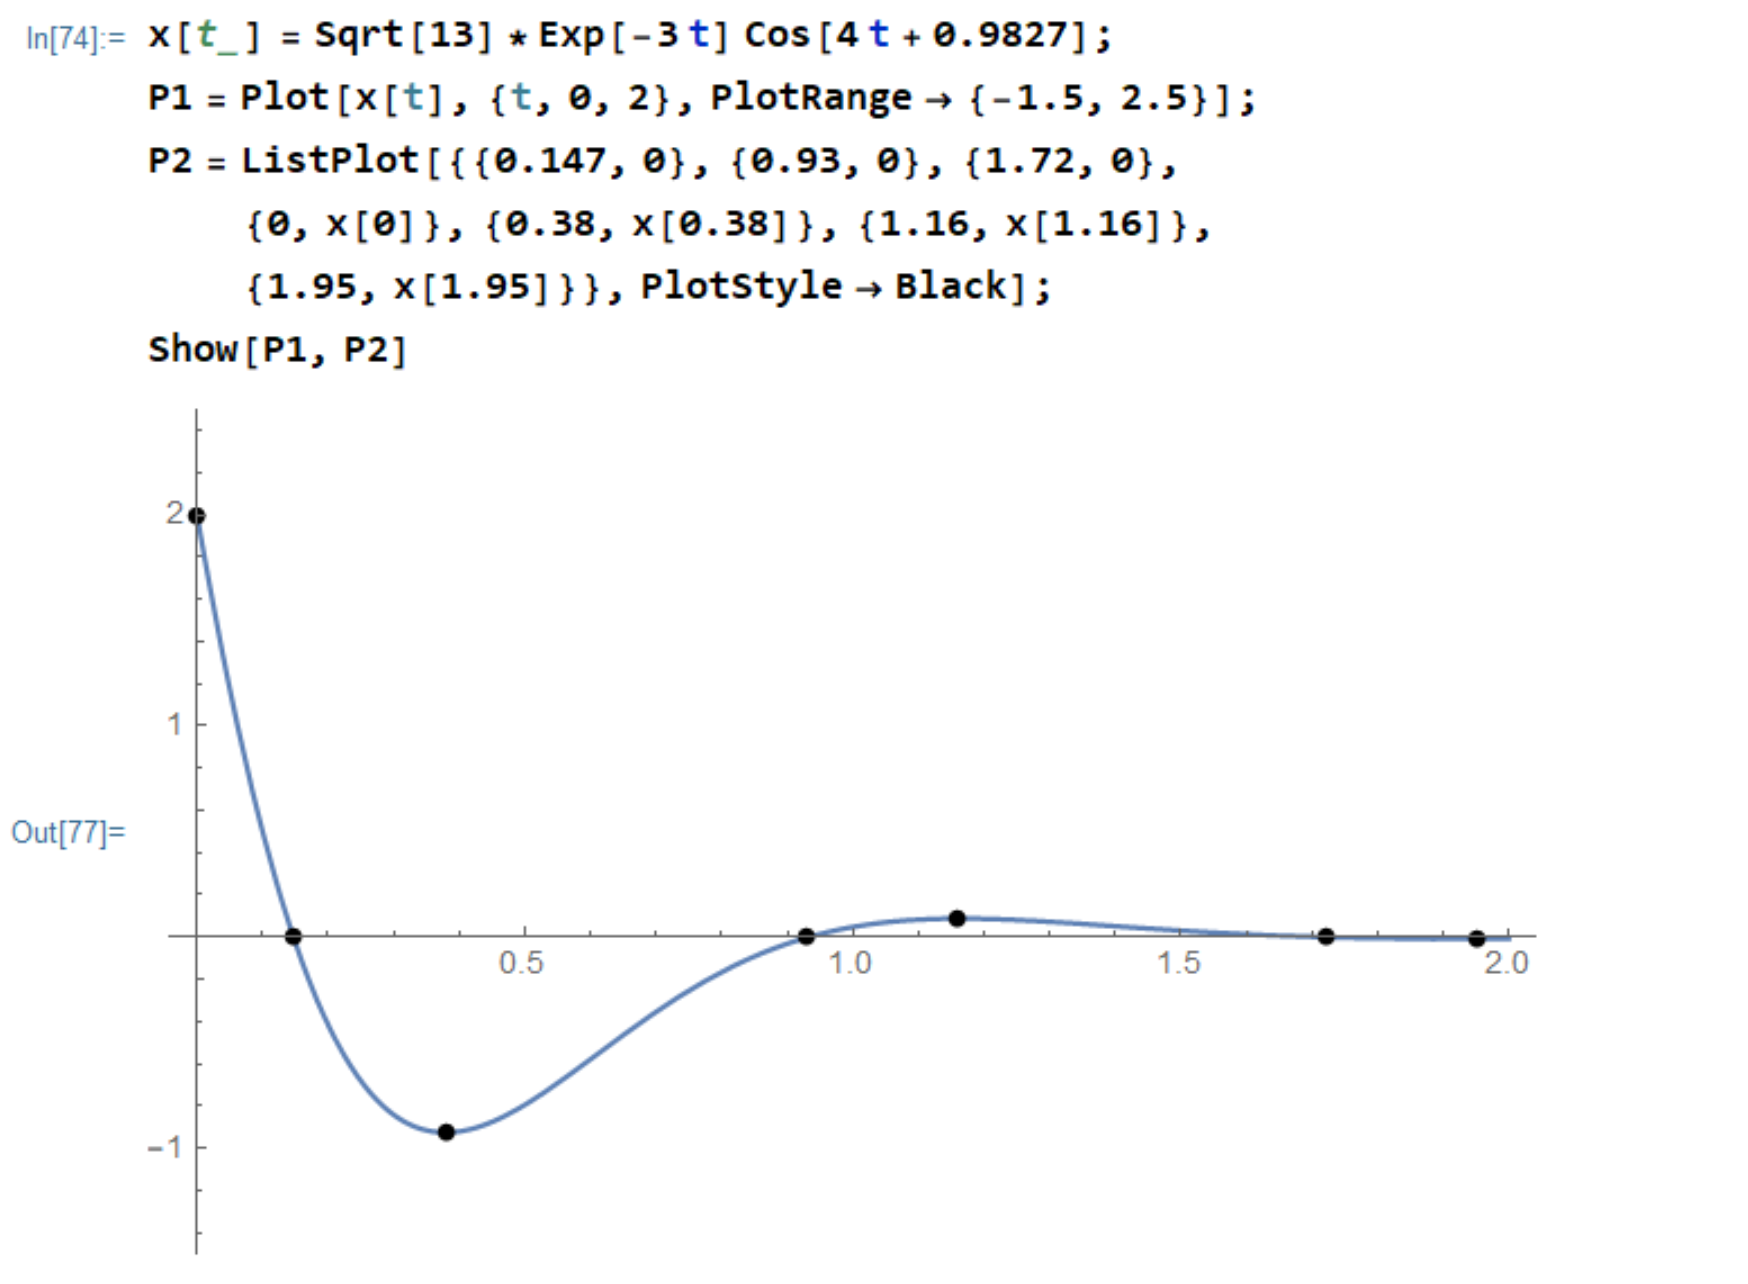
\includegraphics[scale=0.7]{Exam2Graph.PNG}
\end{center}


\end{document}
